\documentclass{beamer}
\usepackage{graphicx}
\usepackage{amsmath}
\usepackage{listings}
\usepackage{xcolor}
\usepackage{tikz}
\usepackage{pgfplots}
\pgfplotsset{compat=1.17}

\usetheme{CambridgeUS}
\title{Introduction to C Programming}
\author{K. V. Vidyasagar}
\date{\today}

% Custom settings for C code
\lstset{
    language=C,
    basicstyle=\ttfamily\small,
    keywordstyle=\color{blue},
    commentstyle=\color{green!50!black},
    stringstyle=\color{red},
    numbers=left,
    numberstyle=\tiny\color{gray},
    stepnumber=1,
    numbersep=8pt,
    frame=single,
    showspaces=false,
    showstringspaces=false,
    tabsize=4
}

\begin{document}

\frame{\titlepage}

\section{Introduction}
\begin{frame}{Introduction}
    \begin{itemize}
        \item C is a general-purpose programming language developed in the early 1970s by Dennis Ritchie at Bell Labs.
        \item Renowned for its efficiency and versatility, C is foundational to many modern programming languages.
        \item Nearly 50 years after its inception, C continues to play a critical role in software development.
    \end{itemize}
\end{frame}

\section{Applications of C}
\begin{frame}{Applications of C}
    \begin{itemize}
        \item Development of operating systems (e.g., UNIX, Windows, Linux).
        \item Programming language interpreters and compilers (e.g., Python interpreter, GCC).
        \item Databases (e.g., Oracle Database, MySQL).
        \item System-level software and embedded systems.
    \end{itemize}
    \begin{center}
        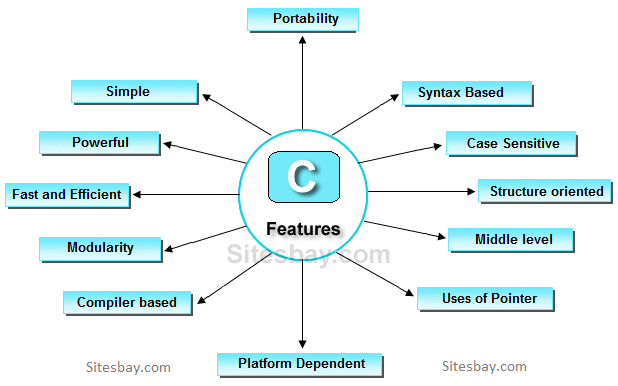
\includegraphics[width=0.8\textwidth]{applications_of_c.png} % Replace with your actual image file
    \end{center}
    \pause
    \textbf{Note:} Ensure the image file \texttt{applications\_of\_c.png} is available in the working directory.
\end{frame}

\section{Key Features of C}
\begin{frame}{Key Features of C}
    \begin{itemize}
        \item \textbf{Procedural Language:} Focuses on functions and procedure calls.
        \item \textbf{Low-Level Access:} Allows direct interaction with hardware.
        \item \textbf{Portability:} Code written in C can be compiled on various platforms.
        \item \textbf{Efficiency:} Generates optimized machine code.
    \end{itemize}
\end{frame}

\section{Basic Structure of a C Program}
\begin{frame}[fragile]{Basic Structure of a C Program}
    Below is an example of a simple C program:
    \begin{lstlisting}
#include <stdio.h>  // Include standard input-output header

int main() {
    // Print a message to the console
    printf("Hello, World!\n");
    return 0; // Return 0 to indicate successful execution
}
    \end{lstlisting}
\end{frame}

\section{Visualization: C Program Flow}
\begin{frame}{Visualization: C Program Flow}
    \begin{center}
        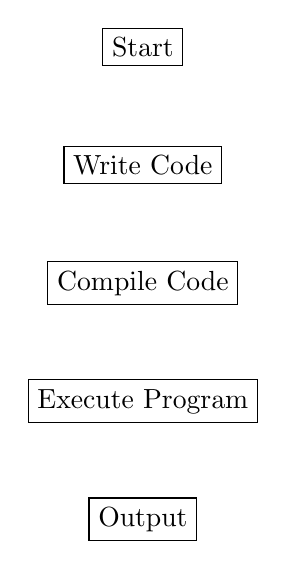
\begin{tikzpicture}[node distance=1.5cm, auto]
            \node[draw, rectangle] (start) {Start};
            \node[draw, rectangle, below of=start] (code) {Write Code};
            \node[draw, rectangle, below of=code] (compile) {Compile Code};
            \node[draw, rectangle, below of=compile] (execute) {Execute Program};
            \node[draw, rectangle, below of=execute] (output) {Output};
            \path[->] (start) -- (code);
            \path[->] (code) -- (compile);
            \path[->] (compile) -- (execute);
            \path[->] (execute) -- (output);
        \end{tikzpicture}
    \end{center}
    \caption{Flow of a C Program}
\end{frame}

\section{Memory Management in C}
\begin{frame}{Memory Management in C}
    \begin{itemize}
        \item C provides manual control over memory using pointers and functions such as \texttt{malloc}, \texttt{calloc}, and \texttt{free}.
        \item The following image illustrates the memory layout of a typical C program.
    \end{itemize}
    \begin{center}
        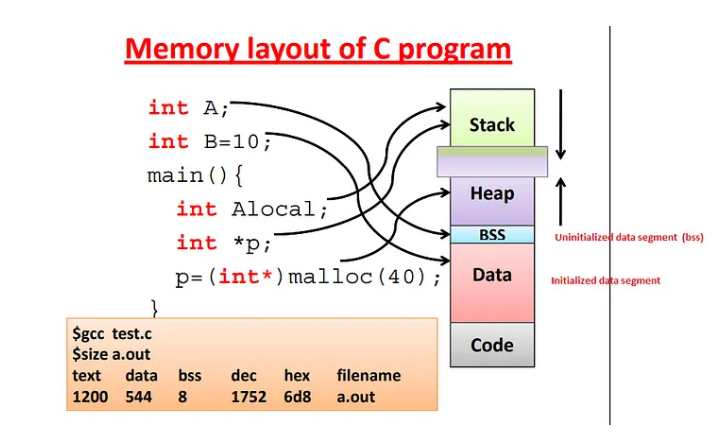
\includegraphics[width=0.8\textwidth]{memory_layout.png} % Replace with your memory layout figure
    \end{center}
    \pause
    \textbf{Note:} Verify the image file \texttt{memory\_layout.png} exists in the working directory.
\end{frame}

\section{Graph: Popularity of C Over Time}
\begin{frame}{Graph: Popularity of C Over Time}
    \begin{center}
        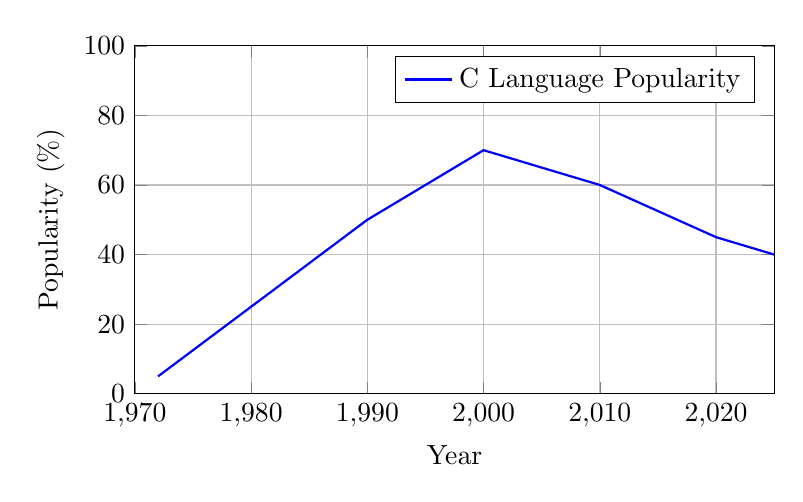
\begin{tikzpicture}
            \begin{axis}[
                width=0.8\textwidth,
                height=6cm,
                xlabel={Year},
                ylabel={Popularity (\%)},
                xmin=1970, xmax=2025,
                ymin=0, ymax=100,
                grid=both,
                legend pos=north east
            ]
                \addplot[color=blue, thick] coordinates {
                    (1972, 5) (1980, 25) (1990, 50) (2000, 70) (2010, 60) (2020, 45) (2025, 40)
                };
                \legend{C Language Popularity}
            \end{axis}
        \end{tikzpicture}
    \end{center}
    \caption{Popularity of C Language Over Time}
\end{frame}

\section{Conclusion}
\begin{frame}{Conclusion}
    \begin{itemize}
        \item C remains a powerful language that continues to influence the development of modern programming languages and systems.
        \item Its efficiency, portability, and low-level capabilities make it a vital tool for computer scientists and engineers.
        \item Understanding C provides a strong foundation for exploring advanced programming concepts.
    \end{itemize}
\end{frame}

\end{document}
